\documentclass[conference]{IEEEtran}
\usepackage{cite}
\usepackage{amsmath,amssymb,amsfonts}
\usepackage{algorithmic}
\usepackage{graphicx}
\usepackage{textcomp}
\usepackage{xcolor}
\def\BibTeX{{\rm B\kern-.05em{\sc i\kern-.025em b}\kern-.08em
    T\kern-.1667em\lower.7ex\hbox{E}\kern-.125emX}}
\begin{document}

\title{CS485G Midterm 1}

\author{\IEEEauthorblockN{Jonathan Moore}
\IEEEauthorblockA{\textit{College of Engineering} \\
\textit{University of Kentucky}\\
Lexington, Kentucky \\
jdmo242@uky.edu}
\and
\IEEEauthorblockN{Oluwafeyisayo Afolabi}
\IEEEauthorblockA{\textit{College of Engineering} \\
\textit{University of Kentucky}\\
Lexington, Kentucky \\
oaaf222@uky.edu}
\and
\IEEEauthorblockN{Zac Foster}
\IEEEauthorblockA{\textit{College of Engineering} \\
\textit{University of Kentucky}\\
Lexington, Kentucky \\
zachary.foster@uky.edu}
}

\maketitle

\begin{abstract}
This project was to create an application that used the CoreLocation framework to track
and record the users location.
\end{abstract}

\section{Introduction}
The primary purpose of this tutorial was to gain experience using the CoreLocation
framework by creating an application that tracks and logs the users location. As an
extention of this primary purpose, the tutorial also offered a number of other opportunities
to learn about various frameworks and aspects of swift as well as experience in storyboarding
and working in Xcode. Through the app design process we were able to learn more about
table views using the UIKit table view controller feature. Using MapKit, we 
learned how to embed a map into the application as well as add custom points of 
interest to it. Another useful feature we gained experience with was the Codable
protocal, which provides an easy way to allow the app data to be encoded and decoded
for storage. We also learned how to use various features of the CoreLocation 
framework such as CLLocationCoordinate2D.

On top of the features included in the original tutorial, we also added in a few 
addition functions that work with the Yelp Fusion API and are applicable towards 
the application we will be developing for the final project. Adding in these features
provided us with the opportunity to gain an understanding of working with APIs and
using other frameworks and functions within Swift and Xcode that will be beneficial
to us when creating our final application.

\section{Functionality}
For this project, our application function was divided into two main portions:
the functions that came from the tutorial we chose and the functions that we decided
to add into the app. Both of these are discussed in detail below.

As a whole, we tried to develop our app using the principles of Model-View-Controller 
(MVC). The way we accomplished this was by dividing our program in such a way that 
all of the data storage and structures (the Model) are only accessed by the view
controllers (the Controller). The view controllers manipulate that data, 
retrieve new data from outside sources such as the Yelp Fusion API, pass things on
for the user to see (in the View), and retrieve input from the user. A simple
chart of how this works for our app is shown as a function diagram in Figure 1
in the References section.

\subsection{Original Function}

\subsubsection{Baseline App}
The first step of the tutorial was to recreate the baseline application that the
tutorial author had given as a download. Since we were not allowed to download
these materials, we had to create our own version to accomplish the same goal.
To create this, we used the information at the beginning of the tutorial as an
outline on what should be included as a starting point. To start, we had to create
a storyboard that included all of the neccesary elements for the app. This meant 
making a Tab Bar Controller that split into a TableView and MapView scenes. After 
creating those scenes and the appropriate buttons on them, we had to create 
ViewController files for each to handle the operations that needed to be done within
those scenes. Using the MVC pattern, those ViewControllers handle all of "middle man"
work, accessing any data structures and handling interaction with the user. After
creating the ViewControllers, we needed a way to store the data recieved so we created
a class called Location that holds all the needed data about a users location and
a class called LocationStorage that handles storing the data to the local disk.
Creating the LocationStorage class gave us experience with the FileManager feature
of the Foundation framework that makes it very easy to save and load data.

\subsubsection{First Half of Tutorial}
This first half of the tutorial after the baseline app had already been 
created mainly focused on asking for the users permissions in-app to do 
things such as track their location and also send them notifications. To do 
this we simply had to add two special strings to the info.plist file which 
asked the user for permission to track their location. After this, we then 
added some lines of code asking the user for permission to send them notifications 
as our app sends notifications letting the user know when they've logged a new 
location. The next step in the tutorial was choosing the most appropriate locations 
data. To do this we relied on the visit monitoring API which allows us to track 
destinations and has the huge benefit of having low battery impact. The next 
step of the tutorial was to then implement reverse geocoding, which is the 
process of converting coordinates into locations/ real world addresses and 
CoreLocation has a class called CLGeoCoder that does that for us. Finally we 
added functionality that would notify the user with a banner notification when 
a new location was logged. This part of the tutorial exposed us to asking for 
various types of permissions in the info.plist file as well as sending the user 
notifications once a location had been logged.

\subsubsection{Second Half of Tutorial}
The second half of the tutorial primarily focused on the implementation of two
distinct features. The first of these features was the ability to record fake
location data, which is necessary when testing the application on a simulated
device during the development process. This feature was implemented by using
Xcode's location simulation tool and intercepting the program when a visit was
to be recorded and inserting the fake location data instead of actual data.
Fake visits are given a unique label to make them easily identifiable. The second
feature implemented is essential to the app's functionality⁠—the ability to store,
retrieve, and visualize location records. When a visit is recorded, the data is 
encoded into JSON and written to a local file on the device. The data is then 
used to populate both the "Location History" list from the first tab, and to
create an annotation in the map view. On startup, the application loads previously
stored data and repopulates the list and map view.

\subsection{Added Functions}
Overall, our team added three additional features to the application that were not 
originally included in the tutorial. These features focused on adding functionality
that would tie into our final application and that created methods that we could
reuse in our future projects.

\subsubsection{Find Closest Restaurant}
The first additional feature that we added was to allow the user to see the closest
restaurant to them in the map view screen. From a user standpoint, we did this by 
adding a button in the top left of the navigation bar that says "Find Food." When 
pressed, this button will create a pin on the map showing the location of the nearest
restaurant, with the restaurant name and address as the pin's label.

From a coding standpoint, the way that this was implemented took a number of steps.
First, in the main storyboard of the application, we added a navigation bar button
to the top left of the MapView scene named "Find Food". We then linked this button
into the MapViewController.swift file to create an IBAction function called findFood().
Inside of the findFood function, we accomplish several things. The first and 
most significant task is that the function sends a request to the Yelp Fusion API
to recieve a JSON object with a list of all the restaurants close to the users current
application. After retreiving the JSON object, our code then uses the data to populate
a structure named BusinessInfo that holds all of the information retrieved from Yelp
in the same layout as the JSON. Using this structure, the function then calls a separate
function that loops through the list of businesses and finds out which restaurant
is closest to the user's current location. Once it has this business, the findFood
function then creates a custom pin (defined as another class: CustomPin), and then
adds it to the map as a MapKit annotation.

\subsubsection{Linking to external maps app or browser}

The Core Location app and our final app idea are similar in the 
sense that they don't give the user directions to any restaurants that 
are logged in the TableView or that show up on the MapView. Our idea is to 
reroute the user to their local Google maps app when they click on a location 
and if they don't have the app, to then open Google maps up in a browser. This 
is mainly to reduce the strain on our app and so it does not have high impact 
on a battery standpoint. To do this, we will be using the Google maps platform 
API, which is very straightforward to use. To do this we first had to add a 
special LSApplicationQueriesSchemes string to the info.plist file containing 
comgooglemaps and googlechromes. After doing this, a function called OpenGoogleMaps 
will then be implemented that takes the latitude and longitude of the desired 
location and then first checks if the user has the Google maps app on their phone. 
If not, Google maps will be opened in the browser and the current location and 
destination will be pre-filled based on the users current location and the 
destination they selected in the app.

\subsubsection{Providing Additional Restaurant Data}
Previously, when the aforementioned "Find Food" button was pressed, the application
simply created a new annotation on the map, centered at the restaurant's location
and with a title containing the restaurant's name. Ideally, however, our app will
provide more detailed information about the restaurant that was found, especially
considering the Yelp API provides much of this data. Our third addition was to
create an additional pop-up dialog when a restaurant was located, displaying its
name, address, user rating, URL, and so on. This was acheived by creating an
additional view controller in the main storyboard, with views for each of the
appropriate data fields that are to be displayed. Using the main storyboard and
the findFood function, the functionality of the "Find Food" button was modified
to bring up this new dialog when clicked. After a restaurant has been found and the
information is loaded, the data is assigned to the appropriate views in the new view
controller. The user can browse the information and click on the restaurant's URL if
desired, or they can select the back button to return to the map view, where they
can see the location of the restaurant via the new map annotation.

\subsection{Functions to be Used in Final Application}
For the most part, this tutorial served as a way to familiarize ourselves with 
Swift and different frameworks. Most of the features from the original tutorial
will not play much into our final app. The only pieces that may come into play
are the MapView and possibly the Tab Bar Controller. The majority of what will
carry into our final app falls in our added functions. Our final application will
rely heavily on the Yelp API so the part of our current code that calls and parses
the JSON recieved will be reused. Other pieces like linking to Google maps and 
showing Yelp info in a pop-up window will also most likely be reused.

\section{Challenges}

\subsection{Challenges in Tutorial}

\subsubsection{Baseline App}
When recreating the baseline app to start the tutorial, the overall biggest challenge
was trying to recreate what was represented in the tutorial with a relatively small
understanding of Swift. This resulted in having to overcome a variety of syntax errors
and other small mistakes throughout the coding process. Besides these small hurdles,
we also had the challenge of learning and understanding how to properly set up the 
storyboard. Not having much experience with this, it took a while to get the correct 
pieces into the main storyboard and to link them properly into the code.

\subsubsection{First Half of Tutorial}
The main challenge we faced in this part of the tutorial was getting the permission 
banner for tracking the users location to remain on the screen. When the code was 
added to ask for permission and the app was built, the location permission banner 
would only flash on the screen and then disappear, not allowing enough time for the 
user to choose if they wanted to allow the app to track their location or not. This bug 
took a while to figure out and we got the answer from stack overflow. This was happening 
because we created the CLLocationManager instance in the didFinishLaunchingWithOptions 
function and once this function had finished running, the dialog disappeared. The solution 
was to simply raise my CLLocationManager instance from being a method-level variable to a 
class-level variable, so we took it out from the didFinishLaunchingWithOptions function and 
placed it at the top of the AppDelegate class. This made sure that the instance wasn't 
disappearing as soon as it was loaded. 

\subsubsection{Second Half of Tutorial}
As we completed the second half of the tutorial, it seemed as though some sections of the
tutorial were outdated or that important excerpts of the required code were ommitted, as
there were several speedbumps in getting our app to work as the tutorial intended. One of
the most prominant hurdles we encountered in this half appeared after implementing the 
"Fake Visits" feature; when the line "locationManager.allowsBackgroundLocationUpdates"
was run, the application crashed and the SIGABRT signal was raised. Error messages from
the console seemed to imply that the program did not have permissions to utilize location
services in the background. Strangely, the simulated device's location permissions checked
out, and the program's Info.plist file had been modified to include the two keys shown in 
the tutorial, yet the error still occurred. After a few hours of attempting to diagnose 
the issue, we discovered that a third key called UIBackgroundModes, which appears to be 
unmentioned by the tutorial, is needed to modify allowsBackgroundLocationUpdates.
Additionally, the name of this key has changed in recent versions, and is now called 
"Required background modes," which made identifying the issue even more challenging.

After resolving the issues with the fake visits feature and attempting to implement
location data retention, another speedbump was encountered. When clicking the plus
button to add a new location to the list, nothing appeared to be happening and the 
Location History list remained empty. Upon restarting the app, we noticed that the
annotations were being added to the map, but the list was still unpopulated. After a
few hours debugging the program, we couldn't find any inconsistancies in our code, but
we noticed that one of the functions that was responsible for populating the list was
never being called. Eventuall we decided to compare our code with the finalized code
from the tutorial website, and found that there were a few functions in 
TableViewController.swift that we did not have and that did not seem to be given in 
the walkthrough. We added these and found that the aforementioned function was now
being called correctly, but an inconsistency in the name for the Table View's cells
was causing another SIGABRT. After resolving these inconsistencies, the application
began working as intended, and the list displayed the location history correctly.

\subsection{Challenges in Additions}
One large hurdle to overcome when making the extra features was figuring out how
to properly call the Yelp Fusion API and retrieve the data from that. It took a 
great deal of research to find out how to correctly use the URLRequest and URLSession
functions to obtain the JSON file from Yelp. After obtaining the file, another large
challenge to overcome was figuring out how to parse the JSON file and use it contents.
We ended up solving this by creating a struct that correlated directly to the contents
of the JSON, and then used the JSONDecoder class to transfer the contents of the 
JSON into a struct.

Another difficulty came about when trying to create the pop-up containing additional
restaurant information. Originally, our plan was to have a small pop-up window appear
at the bottom of the screen when a restaurant annotation was clicked, and the 
additional data would be displayed there. This proved to be too complicated for the
scope of the tutorial, however, as the process of detecting when an annotation is 
clicked was made very difficult due to our implementation of a unique MKAnnotation
class, and the didSelectAnnotationView funtion did not appear to be working. 
Additionally, there did not seem to be a built in view object for a pop-up window
to display over another view. This is a feature that will ideally be present in our 
final application, so this is an undertaking we will likely look into in the future.

\section{References}
\textbf{Figure 1:} The function diagram for our application\\
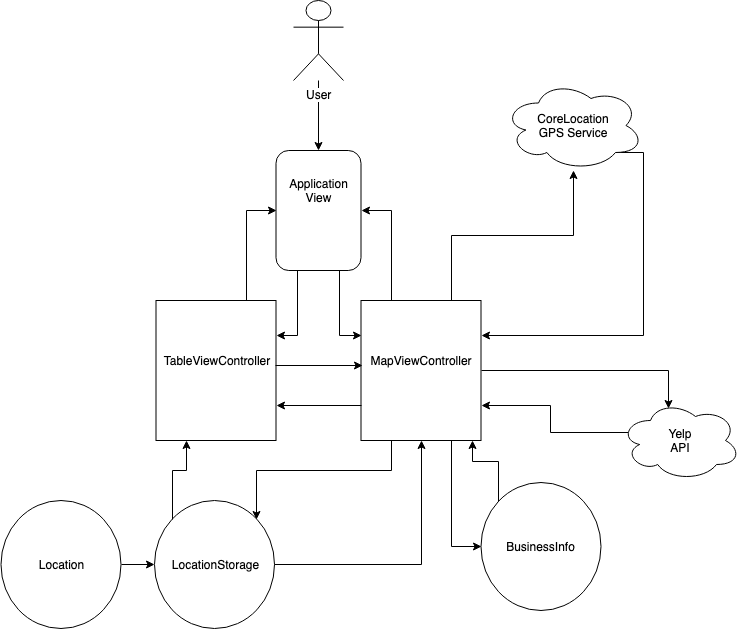
\includegraphics[width=3in]{Midterm1_Function_Diagram.png}

\end{document}
